\documentclass[resume]{subfiles}


\begin{document}
\section{Mémoires}
\begin{itemize}
\item RAM
\item ROM
\item CAM
\item FIFO
\end{itemize}
Amélioration dans le Spartan-6 : LUT4 $\rightarrow$ LUT6 pour de meilleures performances.\\
Les BRAM sont disposées à côté des CLB pour améliorer la vitesse.
\begin{itemize}
\item SliceX (\SI{50}{\percent}) : LUT6, 8 flip-flop
\item SliceL (\SI{25}{\percent}) : + MUX, Carry
\item SliceM (\SI{25}{\percent}) : + distributed RAM, shift register
\end{itemize}
\begin{figure}[H]
\centering
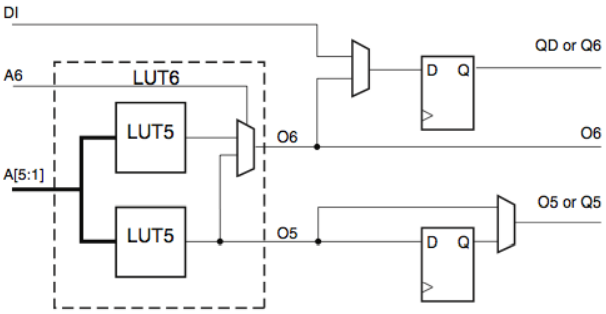
\includegraphics[width=0.6\columnwidth]{img_0.png}
\end{figure}
\subsection{Types de mémoires}
\begin{itemize}
\item On-chip distribuée, utilisation des LUT des CLB (SliceM uniquement).
\begin{itemize}
\item "Granulaire"
\item Peu d'impact sur le routage
\item Petites FIFO / machines d'état
\item \textbf{Rapide}
\item Écriture synchrone, lecture asynchrone (synchrone avec utilisation des flip-flops)
\item Initialisation à la configuration
\item LUT5 = 32 bits. LUT6 = 64 bits.
\item Possibilité de combiner en 256x1, 32x8, etc...
\end{itemize}
\item On-chip block RAM (BRAM)
\begin{itemize}
\item Buffer de moyenne taille
\item \textbf{Rapide}
\end{itemize}
\item Externe
\begin{itemize}
\item Memory Controller Block (MCB)
\item Flexible
\item Très grande capacité
\end{itemize}
\end{itemize}
Toutes les solutions mémoire doivent être rapides et flexibles. Un bitstream doit pouvoir être chargé dans une RAM ou ROM.\\
Example avec un slice contenant 4 LUT6 :
\begin{figure}[H]
\centering
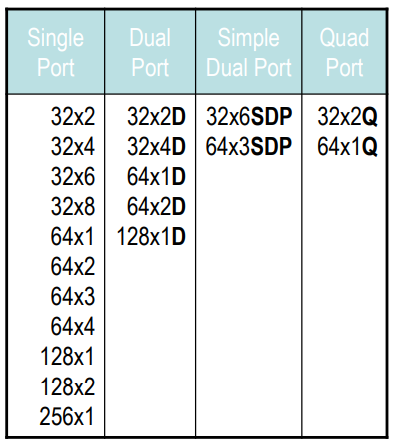
\includegraphics[width=0.4\columnwidth]{img_1.png}
\end{figure}
\subsubsection{Shift register}
SRL16CE ou SRL32 (sur SliceM uniquement)
\begin{itemize}
\item Initialisation possible
\item Chargement impossible
\item Pas de reset
\item Longueur variable (déterminée par l'adresse). Utile pour des buffers dynamiques.
\item Max 128x1 dans une slice (32 par LUT).
\item FIFO synchrone
\item Content-addressable memory (CAM)
\item Générateur de pattern
\item Compensation de délai
\end{itemize}
\subsubsection{BRAM}
Possibilité de
\begin{itemize}
\item Diviser et adresser individuellement les BRAM. 
\item Grouper et adresser de manière unique des BRAM.
\end{itemize}
\begin{itemize}
\item Initialisation possible
\item Reset possible
\item Bits de parité (pour 8 bits de données)
\item Placés à côté des multiplicateurs pour multiply-accumulate
\end{itemize}
$$1\times 18\text{K BRAM}\longleftrightarrow 2\times 9\text{K BRAM}$$
\begin{itemize}
\item True dual port
\begin{itemize}
\item Horloge différente pour chaque port
\item Lecture et écriture synchrone (en même temps)
\end{itemize}
\item Simple dual port
\begin{itemize}
\item Un port en lecture, un port en écriture
\item Lecture et écriture en même temps en 1 cycle
\end{itemize}
\item Single port
\begin{itemize}
\item Lecture OU écriture en 1 cycle
\end{itemize}
\end{itemize}





\subsubsection{Types de mémoires externes}
\begin{itemize}
\item DRAM
\begin{itemize}
\item SDRAM
\item DDR / DDR3
\item FCRAM
\item RLDRAM
\end{itemize}
\item SRAM
\begin{itemize}
\item Sync SRAM
\item DDR SRAM
\item ZBT
\item QDR
\end{itemize}
\item Flash
\item EEPROM
\end{itemize}
\subsection{Implémentation}
\paragraph{RAM distribuée} : Process synchrone, pas de reset asynchrone
\paragraph{Shift register} : Process synchrone, pas de reset asynchrone, serial in et out.


\subsection{Memory Controller Block}
Sur le Spartan-6
\begin{itemize}
\item 4 contrôleurs
\item Mémoires 4, 8 ou 16 bits.
\item Support pour DDR1/2/3, LP DDR
\end{itemize}






\end{document}